\begin{frame}{Hyperparameters}
    \begin{table}[]
    \begin{tabular}{|l|l|}
    \hline
    Hyperparameter          &     Setting              \\ \hline
    Model                   &     Categorical          \\ \hline
    Nodes                   &     120                  \\ \hline
    Layers                  &     6                    \\ \hline
    Dropout                 &     0.65                 \\ \hline
    Batchnormalisation      &     On                   \\ \hline
    Activation              &     elu                  \\ \hline
    Output activation       &     Softmax              \\ \hline
    Batch size              &     1000                 \\ \hline
    Optimisation            &     Adam                 \\ \hline
    Weight Initialisation   &     Lecun Normalisation  \\ \hline
    K-folds                 &     4                    \\ \hline
    \end{tabular}
    \end{table}
\end{frame}

\begin{frame}{Results}
    \begin{columns}
        \begin{column}{0.5\textwidth}
          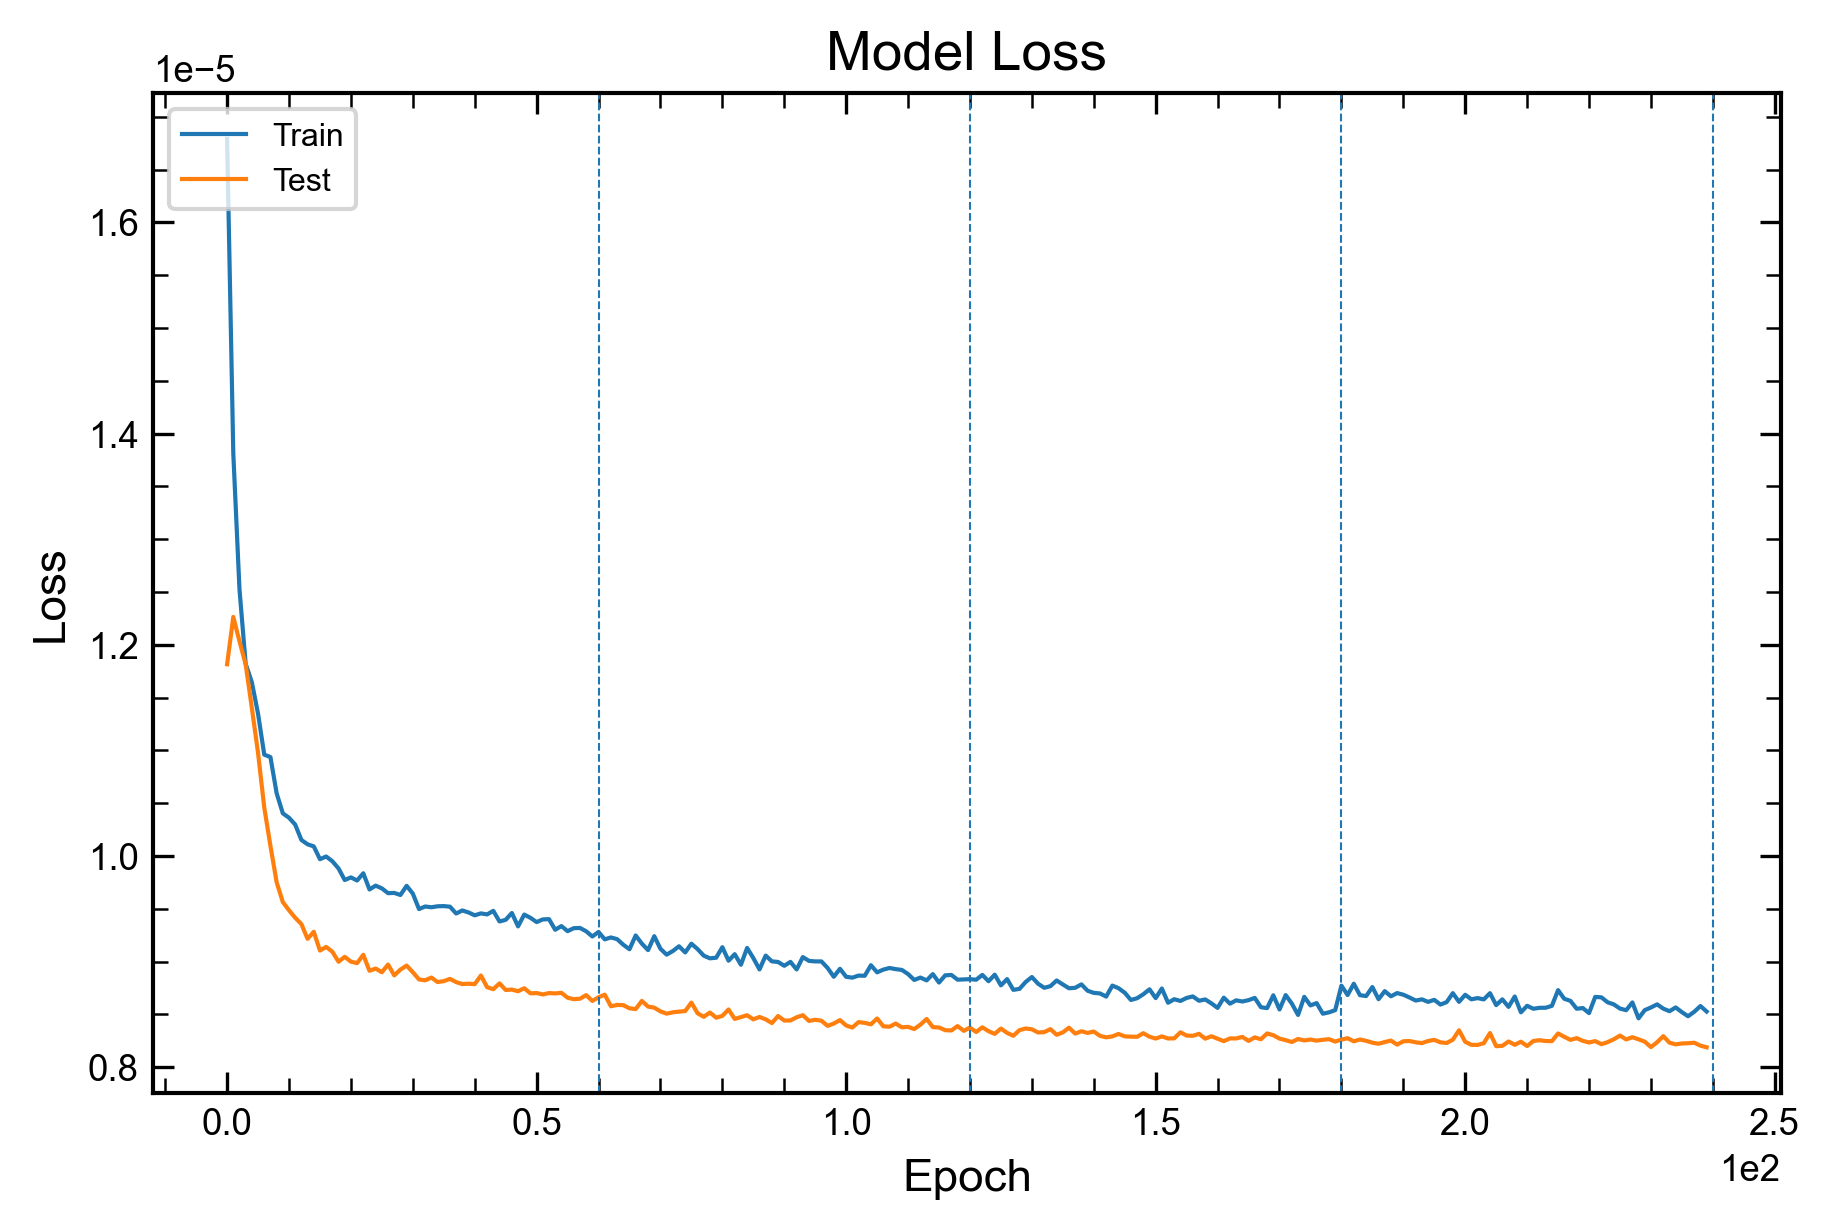
\includegraphics[width=0.8\textwidth]{losses_cat}
          \begin{itemize}
            \item Stable training
            \item Good AUC
          \end{itemize}
        \end{column}
        \begin{column}{0.5\textwidth}
          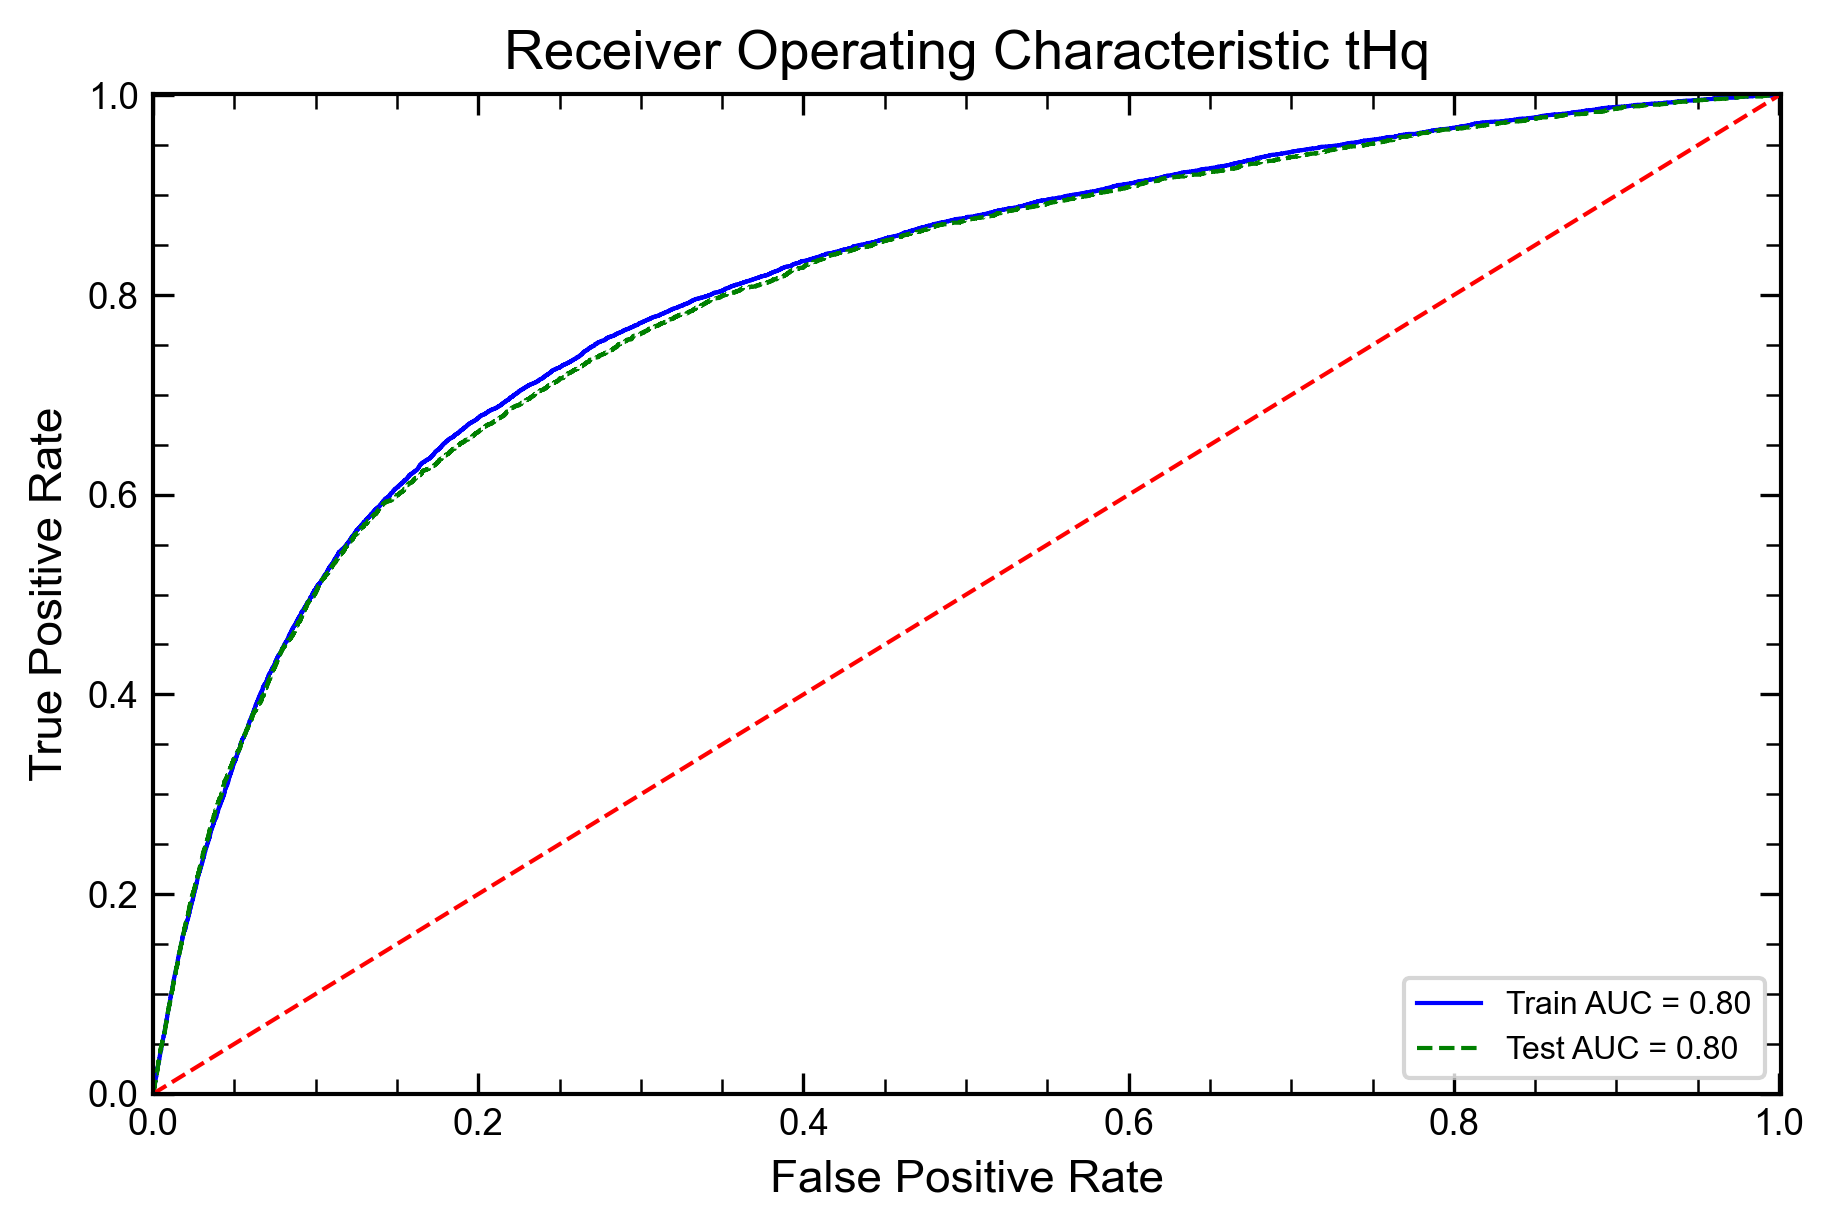
\includegraphics[width=0.8\textwidth]{ROC_cat}
          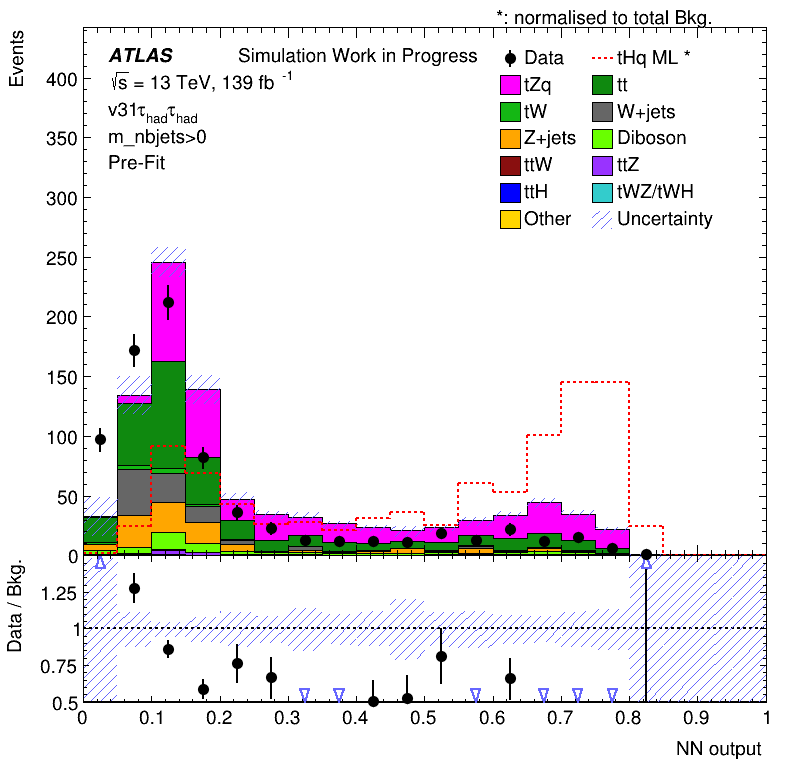
\includegraphics[width=0.8\textwidth]{response_cat}
        \end{column}
    \end{columns}    
\end{frame}

\begin{frame}{Response}
      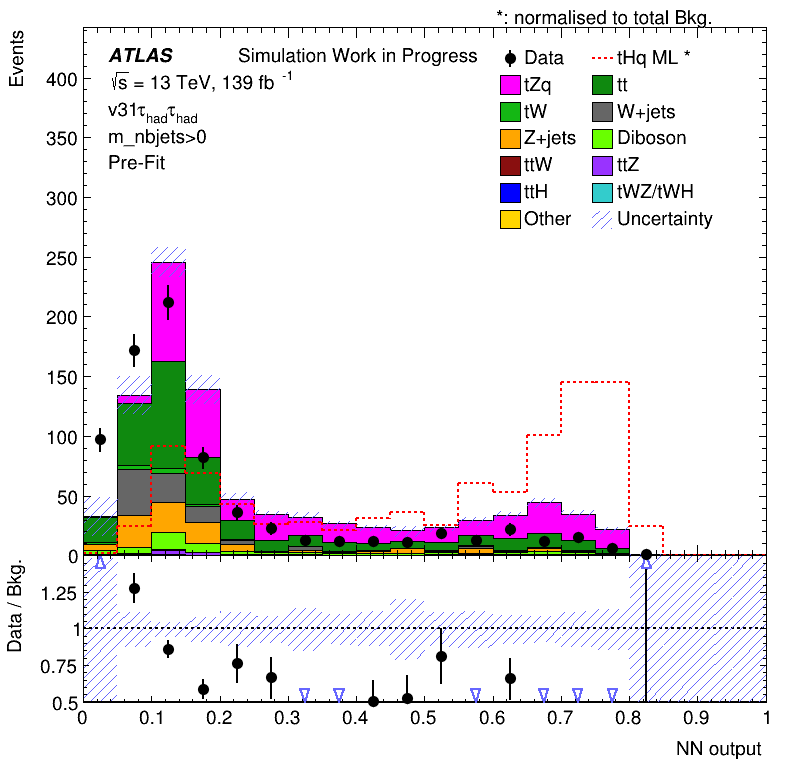
\includegraphics[width=0.75\textwidth]{response_cat}
\end{frame}

\begin{frame}{Additional responses}
  \begin{columns}
    \begin{column}{0.5\textwidth}
      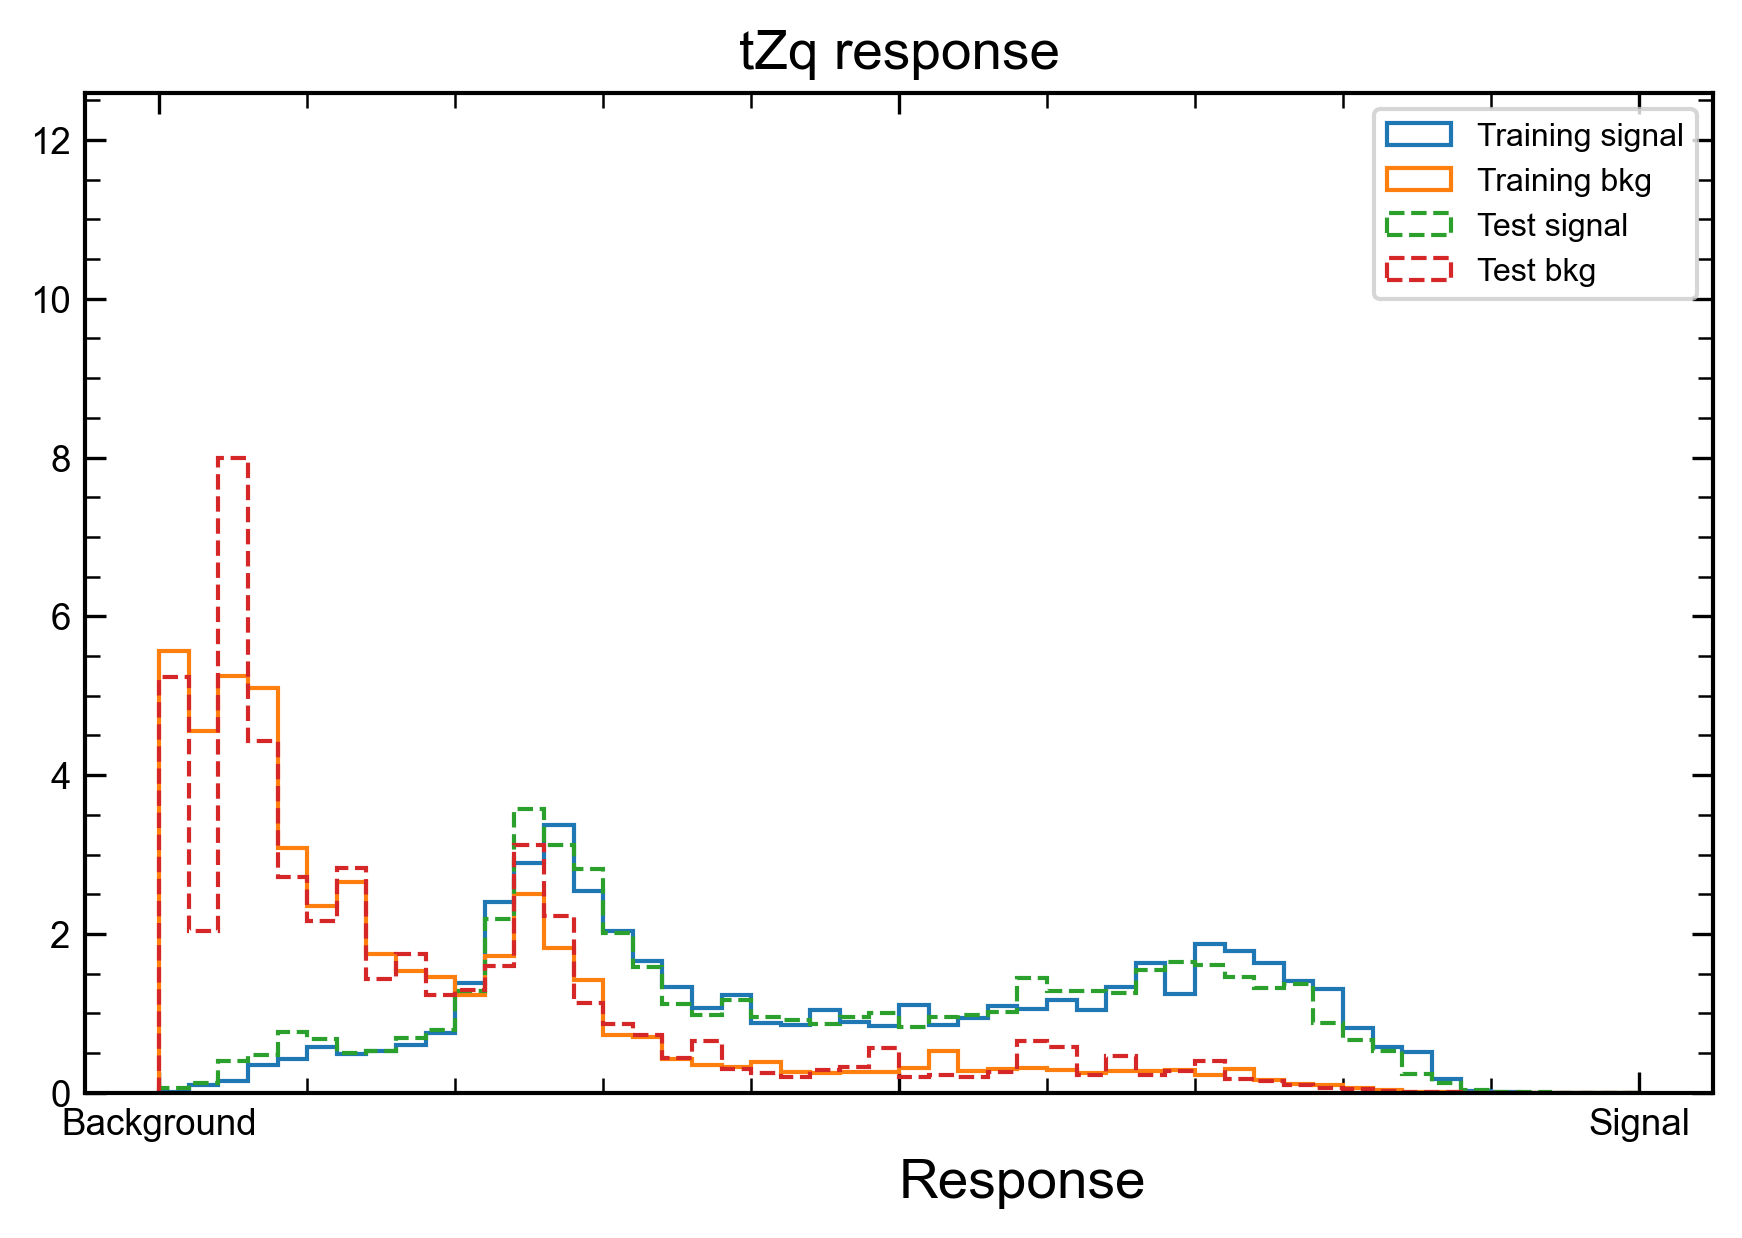
\includegraphics[width=0.8\textwidth]{resp1}
      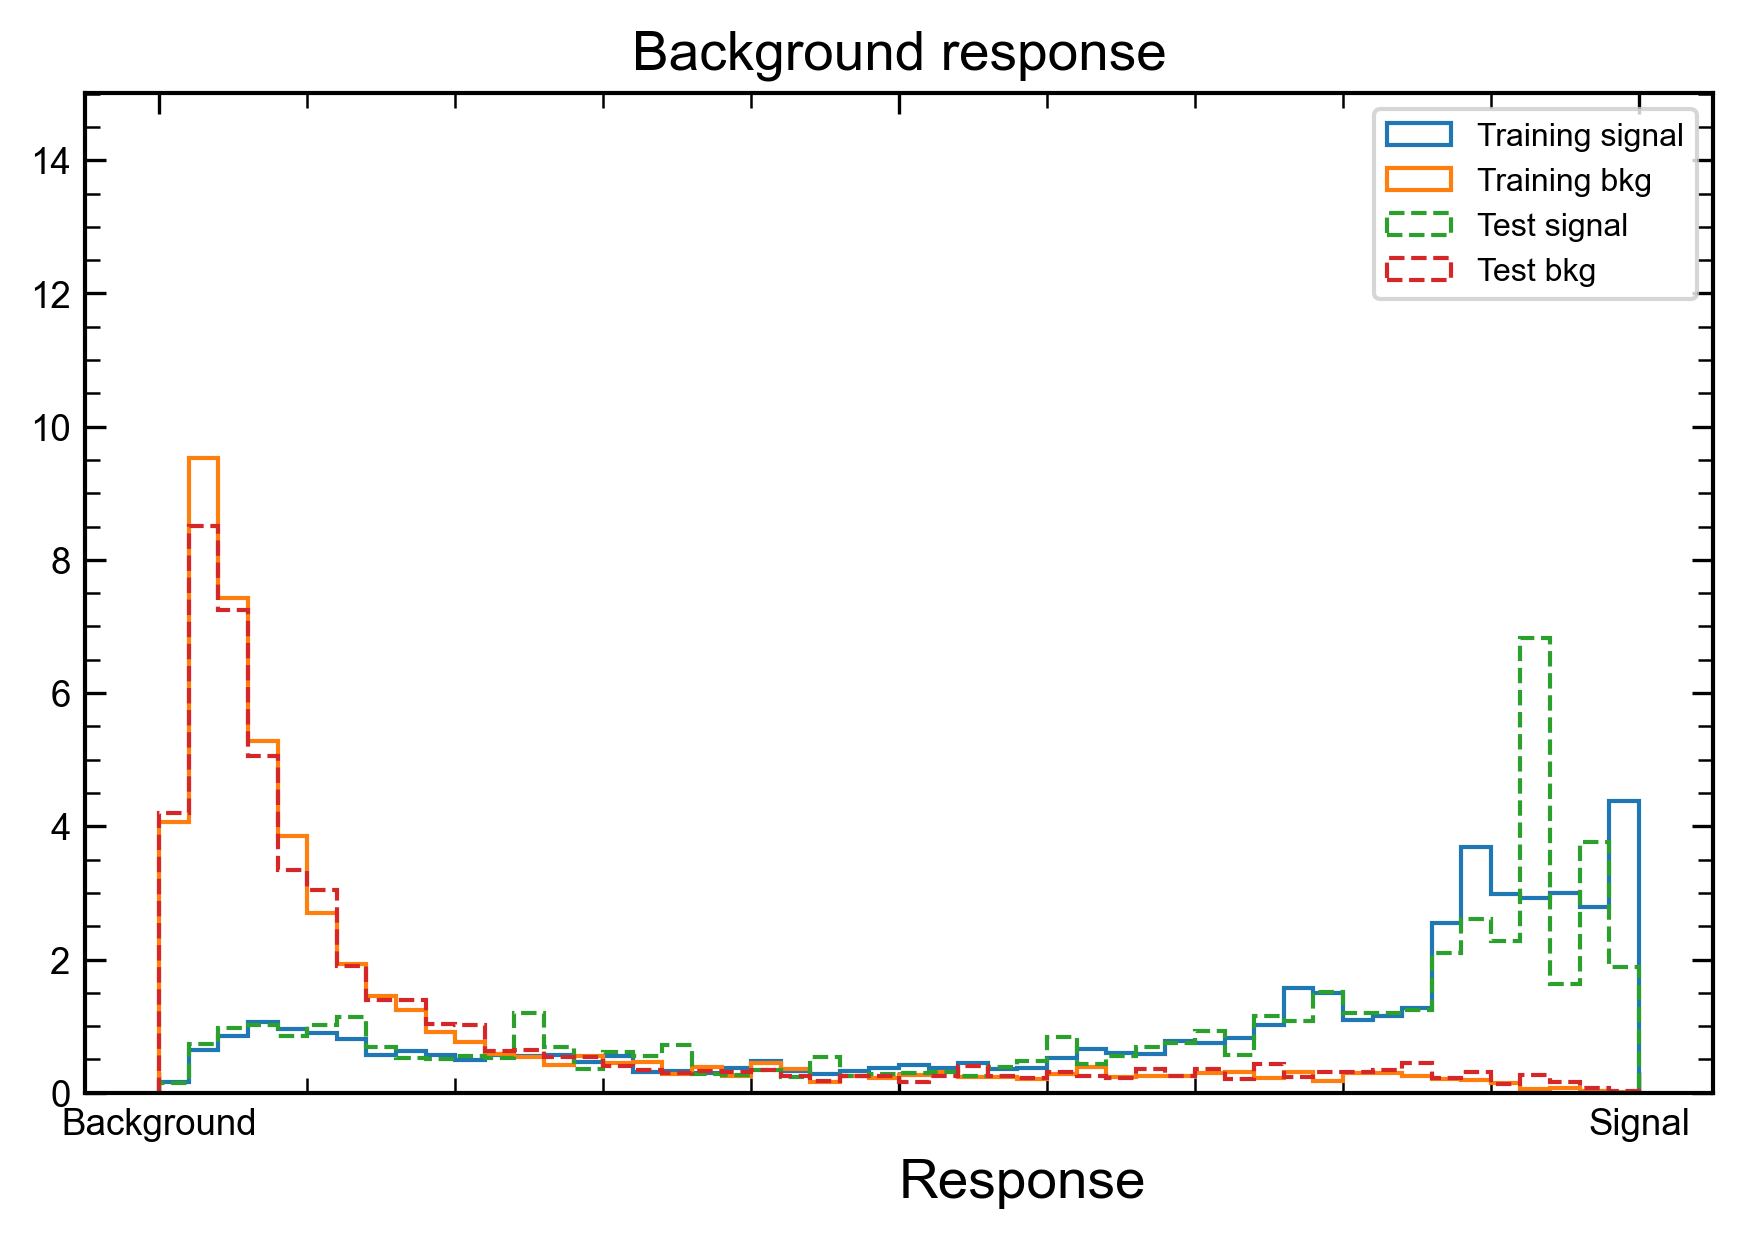
\includegraphics[width=0.8\textwidth]{resp2}
    \end{column}
    \begin{column}{0.5\textwidth}
      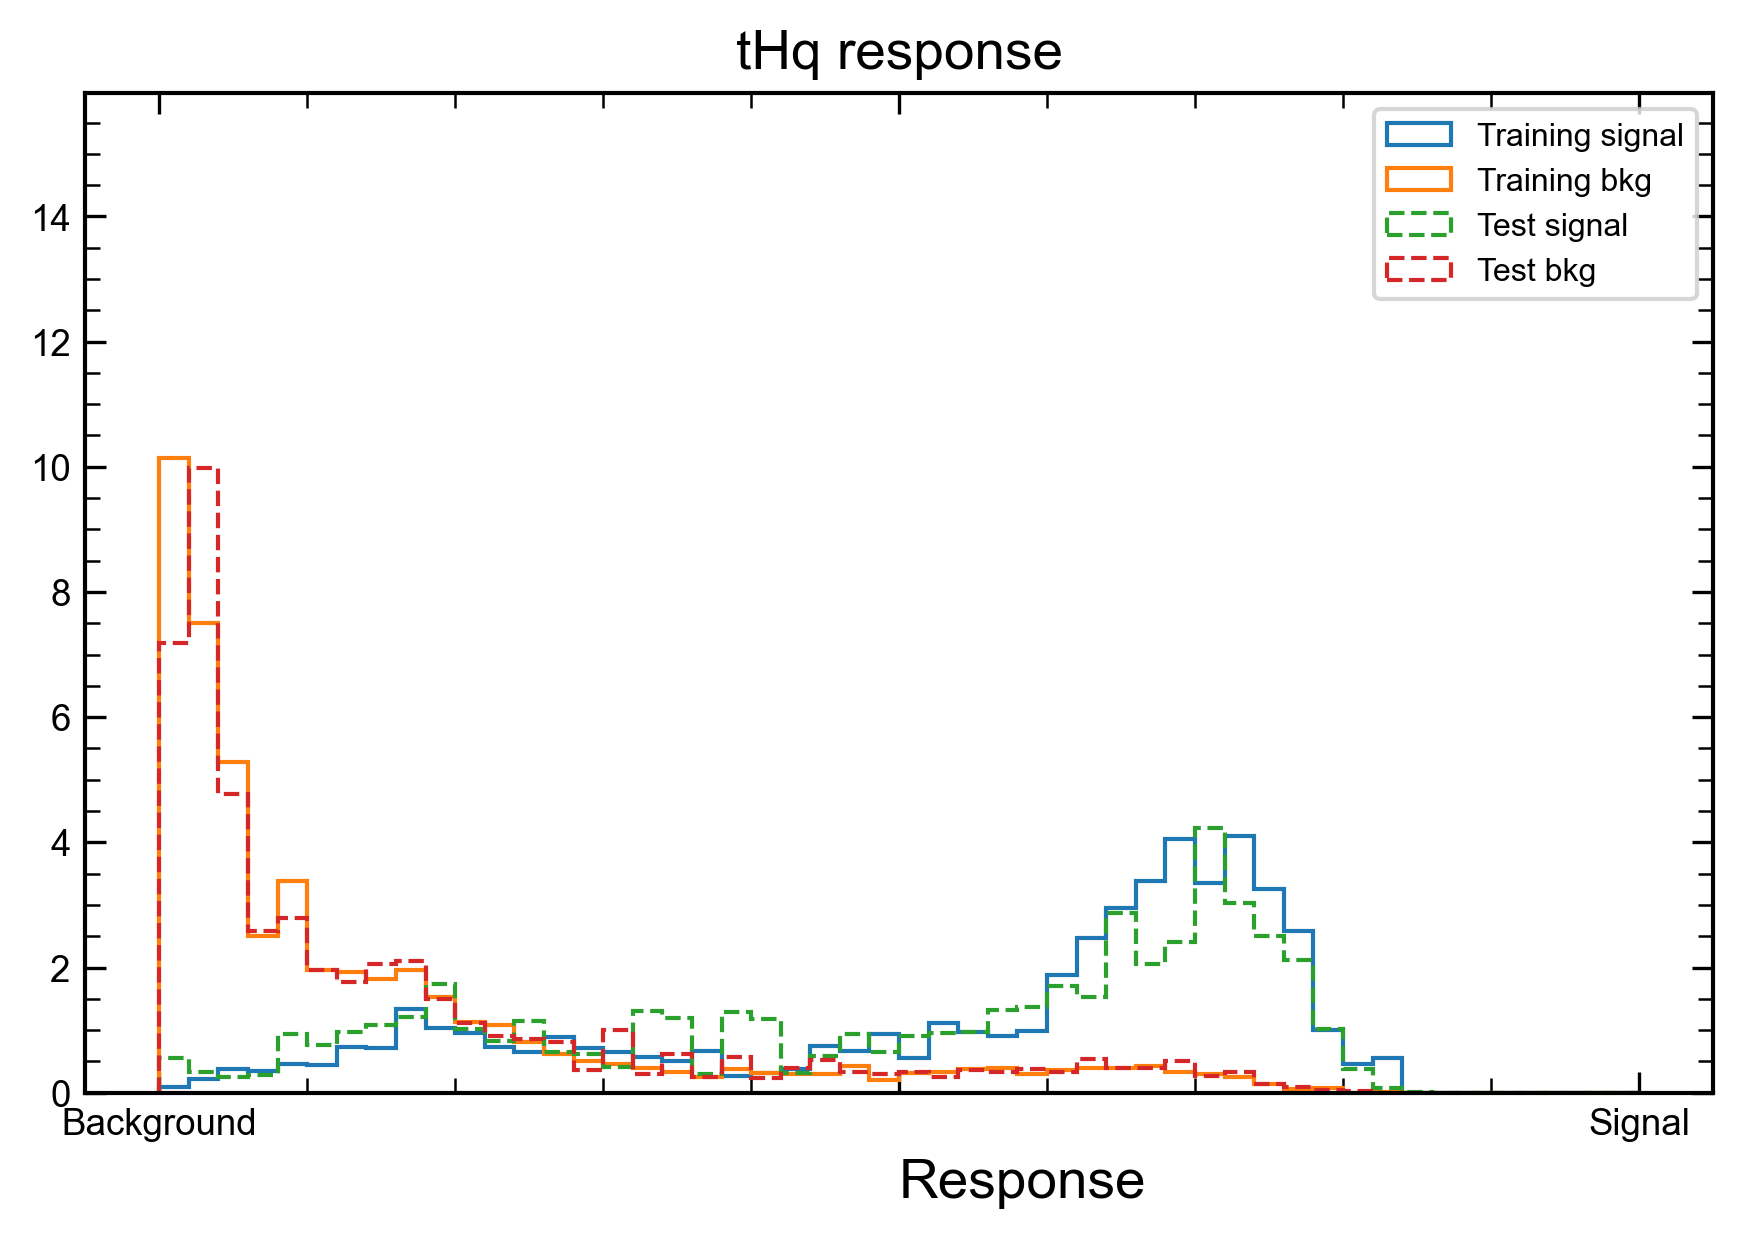
\includegraphics[width=0.8\textwidth]{resp3}
      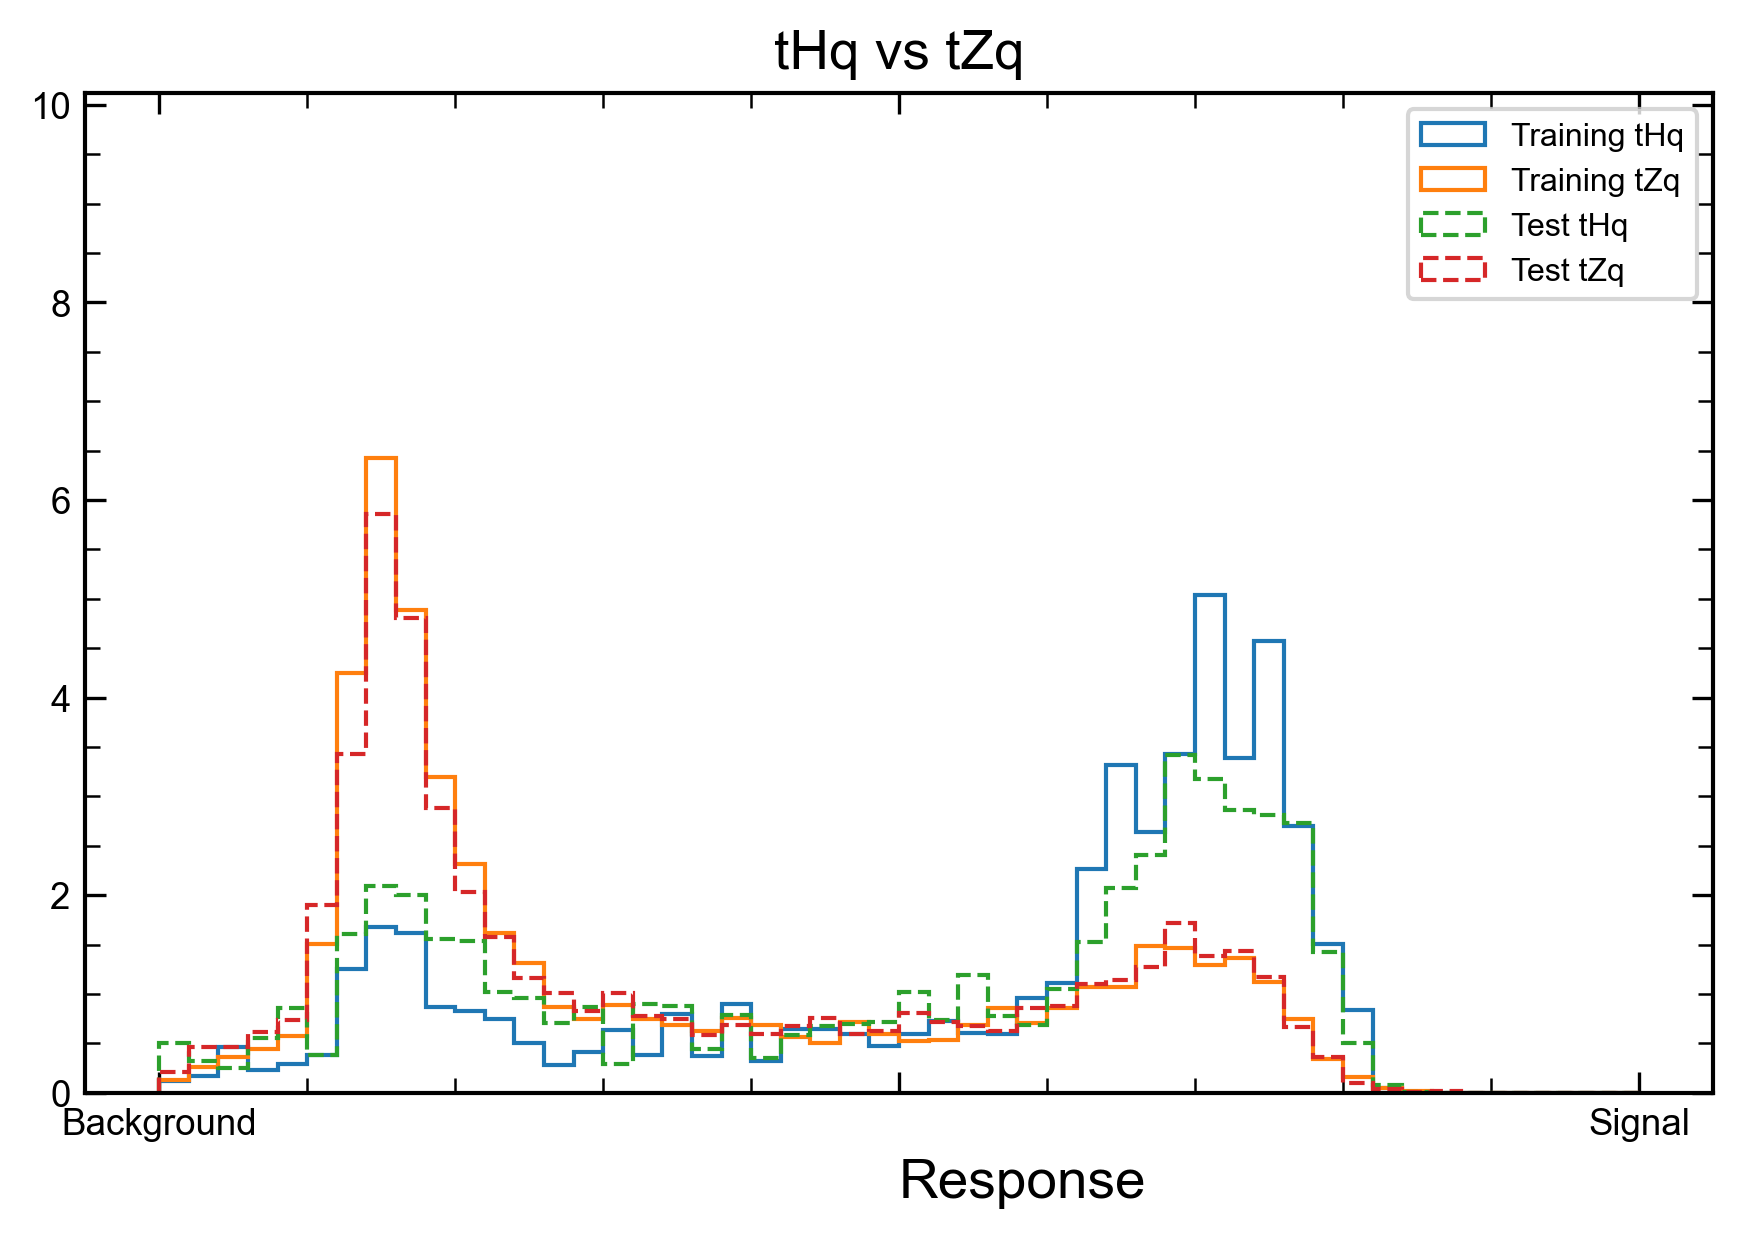
\includegraphics[width=0.8\textwidth]{resp4}
    \end{column}
  \end{columns}    
\end{frame}

